% !TEX TS-program = pdflatex
% !TEX encoding = UTF-8 Unicode

% This file is a template using the "beamer" package to create slides for a talk or presentation
% - Giving a talk on some subject.
% - The talk is between 15min and 45min long.
% - Style is ornate.

% MODIFIED by Jonathan Kew, 2008-07-06
% The header comments and encoding in this file were modified for inclusion with TeXworks.
% The content is otherwise unchanged from the original distributed with the beamer package.

\documentclass{beamer}


% Copyright 2004 by Till Tantau <tantau@users.sourceforge.net>.
%
% In principle, this file can be redistributed and/or modified under
% the terms of the GNU Public License, version 2.
%
% However, this file is supposed to be a template to be modified
% for your own needs. For this reason, if you use this file as a
% template and not specifically distribute it as part of a another
% package/program, I grant the extra permission to freely copy and
% modify this file as you see fit and even to delete this copyright
% notice. 


\mode<presentation>
{
  \usetheme{Warsaw}
  % or ...
  \usecolortheme{beaver}

  \setbeamercovered{transparent}
  % or whatever (possibly just delete it)
}


\usepackage[english]{babel}
% or whatever

\usepackage[utf8]{inputenc}
% or whatever

\usepackage{times}
\usepackage[T1]{fontenc}
% Or whatever. Note that the encoding and the font should match. If T1
% does not look nice, try deleting the line with the fontenc.


\title{Assignment 2}

\subtitle
{Automated Reasoning in AI 2011} % (optional)

\author{Armon Toubman, Torec Luik}

\begin{document}

\begin{frame}
  \titlepage
\end{frame}

%\begin{frame}{Outline}
%  \tableofcontents
%\end{frame}


% Since this a solution template for a generic talk, very little can
% be said about how it should be structured. However, the talk length
% of between 15min and 45min and the theme suggest that you stick to
% the following rules:  

% - Exactly two or three sections (other than the summary).
% - At *most* three subsections per section.
% - Talk about 30s to 2min per frame. So there should be between about
%   15 and 30 frames, all told.

\section{Introduction}

\subsection[General]{General Overview}

\begin{frame}{Sudoku}

\begin{table}[htbp]
\caption{Example of a Sudoku. From the first line of "sudoku\_training.txt". }
    \label{tab:sudoku_initial}
        \begin{tabular}{||c|c|c||c|c|c||c|c|c||}
        \hline
        \hline
         & 9 & 4 &  &  &  & 1 & 3 & \\
        \hline
         &  &  &  &  &  &  &  & \\
        \hline
         &  &  &  & 7 & 6 &  &  & 2\\
        \hline
        \hline
         & 8 &  &  & 1 &  &  &  & \\
        \hline
         & 3 & 2 &  &  &  &  &  & \\
        \hline
         &  &  & 2 &  &  &  & 6 & \\
        \hline
        \hline
         &  &  &  & 5 &  & 4 &  & \\
        \hline
         &  &  &  &  & 8 &  &  & 7\\
        \hline
         &  & 6 & 3 &  & 4 &  &  & 8\\
        \hline
        \hline
        \end{tabular}
    \end{table}
\end{frame}

\begin{frame}{Sudoku as CSP}

  \begin{itemize}
  \item
    Variables   : Unassigned cells.
  \item
    Assignment  : Assigned cells.
  \item
    Domains     : Values 1 to 9.
  \item
    Constraints : Values 1 to 9 once in every row, column, region.
  \item
    Consistency : Constraints not violated.
  \item
    Termination : No variables left.
  \end{itemize}
\end{frame}

\begin{frame}{CSP as tree}

  \begin{figure}[htbp]
\begin{center}
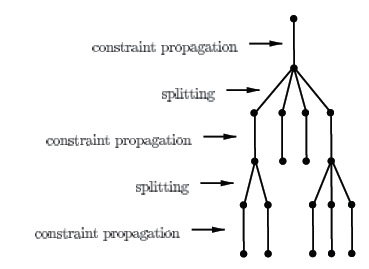
\includegraphics{tree.png}
\caption{Example of a CSP search tree. From Constraint Programming - lecture 3 (CSP) Algorithms. }
\label{fig:basic_tree}
\end{center}
\end{figure}

\end{frame}

\begin{frame}{Make Titles Informative. Use Uppercase Letters.}

  \begin{itemize}
  \item
    Use \texttt{itemize} a lot.
  \item
    Use very short sentences or short phrases.
  \end{itemize}
\end{frame}

\begin{frame}{Make Titles Informative.}

  You can create overlays\dots
  \begin{itemize}
  \item using the \texttt{pause} command:
    \begin{itemize}
    \item
      First item.
      \pause
    \item    
      Second item.
    \end{itemize}
  \item
    using overlay specifications:
    \begin{itemize}
    \item<3->
      First item.
    \item<4->
      Second item.
    \end{itemize}
  \item
    using the general \texttt{uncover} command:
    \begin{itemize}
      \uncover<5->{\item
        First item.}
      \uncover<6->{\item
        Second item.}
    \end{itemize}
  \end{itemize}
\end{frame}


\subsection{Second Subsection}

\begin{frame}{Make Titles Informative.}
\end{frame}

\begin{frame}{Make Titles Informative.}
\end{frame}



\section*{Summary}

\begin{frame}{Summary}

  % Keep the summary *very short*.
  \begin{itemize}
  \item
    The \alert{first main message} of your talk in one or two lines.
  \item
    The \alert{second main message} of your talk in one or two lines.
  \item
    Perhaps a \alert{third message}, but not more than that.
  \end{itemize}
  
  % The following outlook is optional.
  \vskip0pt plus.5fill
  \begin{itemize}
  \item
    Outlook
    \begin{itemize}
    \item
      Something you haven't solved.
    \item
      Something else you haven't solved.
    \end{itemize}
  \end{itemize}
\end{frame}


\end{document}


